\section{General Theory}
\subsection{Image processing}
Image processing is a method of performing operations on an image to extract information or enhance its features. It is a broad field that covers a range of techniques, including image acquisition, Pre-processing, segmentation, feature extraction, image analysis, and visualization. In general, image processing involves transforming an image into a more useful form for analysis or display. This can be achieved through a variety of techniques, such as filtering, edge detection, Thresholding, and morphological operations. Image processing has numerous applications in various fields, including medicine, remote sensing, surveillance, robotics, and entertainment. \cite{wilhelm2016digital}, \cite{tyagi2018understanding} 

\subsection{Deep Learning and Neural Networks}
Deep learning is another name for a multilayer artificial neural network or multilayer perceptron. The elementary
bricks of deep learning are the neural networks, that are combined to form the deep neural networks.

\begin{table}[htbp]
\centering
\caption{Comparing Neural Networks and Deep Learning}
\footnotesize
\begin{tabular}{ |p{3cm}|p{5cm}|p{5cm}| }%{ |c|c|c| }
\hline
Feature & Neural Networks & Deep Learning \\
\hline
Structure & Single-layer or shallow neural networks (typically two to three layers) & Deep neural networks with multiple layers (typically more than three) \\
\hline
Learning Ability & Can learn simple patterns and make predictions & Can learn complex patterns, including abstract relationships, and make more accurate predictions \\
\hline
Data Requirements & Requires less training data & Requires more training data to learn complex patterns patterns \\
\hline
Computational Cost & Less computationally expensive & More computationally expensive, especially for deep neural networks with many layers \\
\hline
Applications & Image classification, fraud detection, spam filtering & Image recognition, natural language processing, speech recognition, medical diagnosis, self-driving cars \\
\hline
\end{tabular}
\end{table}

The term "deep" in deep learning refers to the use of multiple layers in the neural network. Deep learning models, often called deep neural networks (DNNs), are capable of learning and representing complex patterns and hierarchical features from data. \cite{nielsen2015neural} \cite{Arnold2011AnIT}, \cite{2015Natur.521..436L} \\

Various types of deep learning systems exist, distinguished by their neural network architectures and operational principles. Examples include feed-forward neural networks, convolutional networks, recurrent neural networks, autoencoders, and deep beliefs. These methodologies have facilitated substantial advancements in sound and image processing domains, encompassing tasks such as facial recognition, speech recognition, computer vision, automated language processing, and text classification (e.g., spam detection). The potential applications of these techniques are diverse. An illustrative instance is the AlphaGo program, which achieved world champion status in the game of Go in 2016 by leveraging deep learning methodologies.\cite{koons2005}, \cite{shinde2018review}, \cite{choi2020introduction}
\begin{figure}[H]
    \centering
    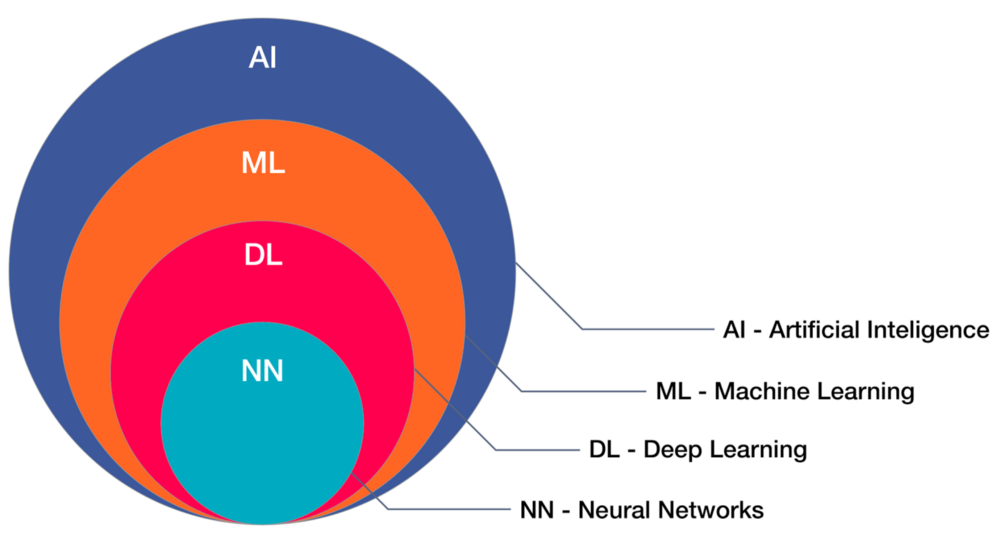
\includegraphics[width=0.8\linewidth]{tex/img/NN_DL_ML.png}
    \caption{Neural network core of deep learning \cite{an}}
    \label{fig:NN_DL}
\end{figure}

\subsection{Neural Networks}
Neural networks are the fundamental components of deep learning. They are composed of layers of interconnected nodes or neurons that process information.
Artificial neural networks (ANNs) are computing systems that are designed to work in a similar way to the human brain.

\subsubsection{The Biological Inspiration}
The complexity of the brain has made it challenging for scientists to fully understand it, despite extensive research. Engineers have modified neural models to create a more useful and less biological approach, while still maintaining much of the original terminology.
\begin{figure}[H]
    \centering 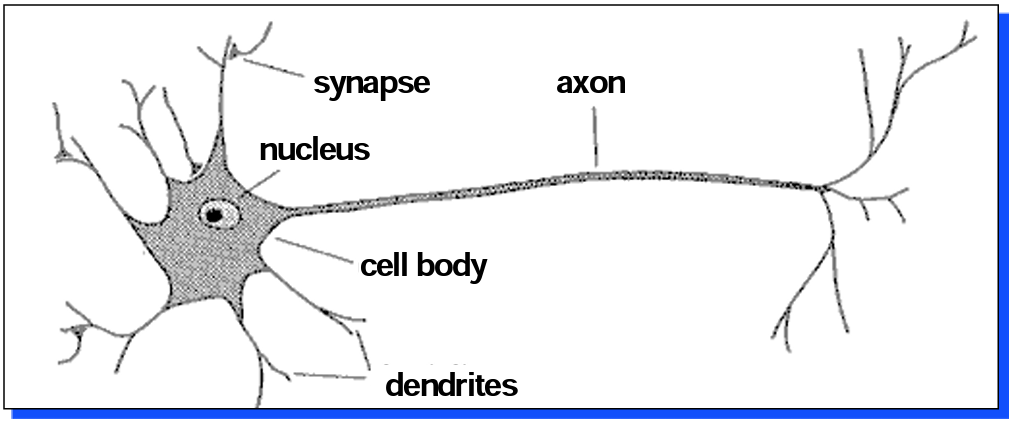
\includegraphics[width=0.5\linewidth]{tex/img/Structure_of_Neurons.PNG}
    \caption{The structure of Neurons \cite{nielsen2015neural}}
    \label{fig:Neuron structure}
\end{figure}
A neuron is composed of three main parts - the cell body, the dendrite (which branches out to receive input), and the axon (which branches out to send output). Connections between axons and dendrites are made via synapses. Electro-chemical signals are carried from the dendrites, through the cell body, and down the axon to other neurons.


\subsubsection{Perceptron}
A single neuron of a neural network is called a perceptron. A perceptron implements a mathematical function that operates on the input signals and generates outputs. Figure is an example of a perceptron. A perceptron is the simplest neural network.
\subsubsection{The learning process}
A perceptron model starts by multiplying all the input values and their weights and then sums these values to create a weighted sum. This weighted sum is then applied to the activation function "f" to obtain the desired result. This activation function is also known as a step function and is represented by "f". This step function or activation function plays an essential role in ensuring that the output signal is mapped between the required values (0,1) or (-1,1). Please note that the weight of the input data indicates the strength of the node. similarly, the value of the input bias allows the activation function curve to shift up or down.
The input signals to a neuron come either from a source (a camera or sensing device) or from the outputs of other neurons.

\begin{figure}[H]
    \centering
    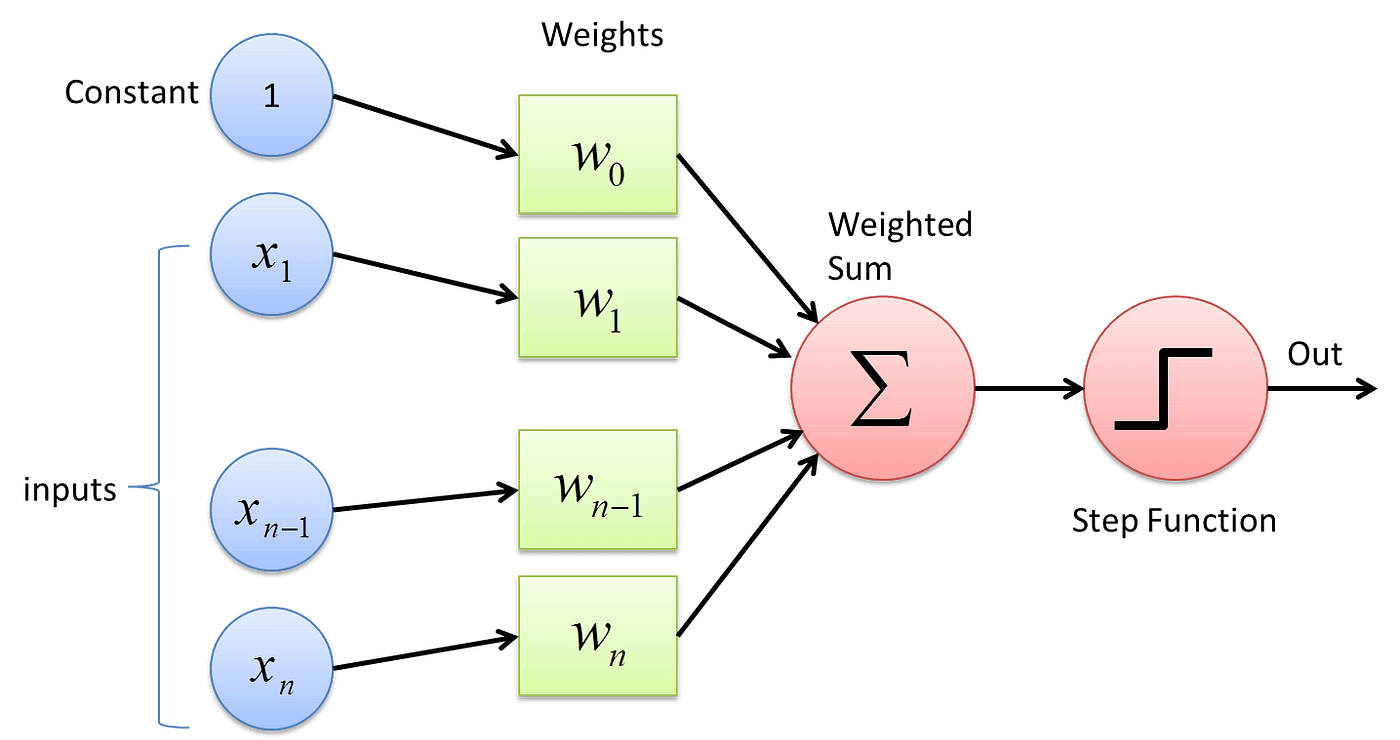
\includegraphics[width=0.7\linewidth]{tex/img/Perceptron.png}
    \caption{Perceptron}
    \label{fig:Perceptron}
\end{figure}

Mathematically, the output (y) of a neuron in a neural network perceptron can be expressed as:\\

\(y=f(\sum_{i=1}^{n}(\omega_{i}.x_{i})+b)\)

where:\\
$\omega_{i}$ is the weight associated with the input \(x_{i}\)\\
\(b\) is the bias term,\\
\(f:\) activation\\
As shown in fig \ref{fig:Perceptron}, One percepteron has the following components: \\
\begin{itemize}
    \item \textbf{Input Nodes or Input Layer: }  
    The input layer, also called input nodes, is the first layer of a neural network. It is responsible for receiving input data, which can be any numerical values, images or text. The input layer does not perform any calculations or transformations of the input data, but only forwards them to subsequent layers in the network. \cite{ansari2020building}, \cite{nielsen2015neural}\\
    \item \textbf{Weight: } Weights are parameters that adjust the strength of the connections between neurons (nodes) in adjacent layers of a neural network. Each connection has an associated weight, and these weights are learnable and updated during the training process. The weights determine the impact of the input signals on the neurons in the next layer. A higher weight means that the corresponding input has a stronger influence on the neuron's output. During training, the neural network adjusts these weights to minimize the difference between the predicted output and the actual target output. \\
    \item \textbf{Bias: } Biases are additional parameters in a neural network that allow for fine-tuning the output of each neuron. Unlike weights, biases are not associated with specific inputs but are added to the weighted sum of inputs in each neuron.
    Role: Biases provide the neural network with flexibility, enabling it to account for situations where all inputs are zero or have low values. They allow neurons to activate even when the weighted sum of inputs is not sufficient to trigger an output.Like weights, biases are adjusted during training to improve the overall performance of the network. \cite{ansari2020building}, \cite{nielsen2015neural}\\
    \item \textbf{Activation Function: } The primary purpose of an activation function is to determine whether a neuron should be activated (output a signal) or not, based on the input it receives.
    An activation function is a mathematical operation enacted on the output of a neuron (or node) within the architecture of a neural network. It introduces non-linearity to the network, allowing it to learn complex patterns and make more sophisticated decisions. The activation function takes the weighted sum of inputs and a bias term and produces the output of the neuron.\cite{nielsen2015neural}

\end{itemize}
\subsubsection{Types of Perceptron: }
Based on the layers, Perceptron models are divided into two types.
\begin{enumerate}
    \item \textbf{Single-layer perceptron model:}  This is one of the simplest types of artificial neural networks (ANN). The single-layer perceptron model consists of a feedforward network and also includes a threshold transfer function inside the model. The main goal of the single-layer perceptron model is to analyze linearly separated objects with binary outputs.

    In a single-layer perceptron model, its algorithms do not contain recorded data, so it starts with a non-constantly allocated input for weight parameters. Furthermore, it sums all inputs (weight). If, after adding all inputs, the sum of all inputs is greater than the set value, the model will be activated and display the output value as +1.
    If the result is the same as the previously established threshold value, then the performance of this model is considered satisfactory and the weight requirements do not change. However, this model contains several discrepancies that arise when many input weight values are introduced into the model. Therefore, some changes should be necessary when entering the weights to find the desired result and minimize errors.
    A single-layer perceptron learns patterns that can be solved linearly. \cite{ansari2020building}, \cite{knerr1990single}

        \item \textbf{Multi-layer Perceptron} An artificial neural network, similar to the human brain, comprises several neurons, also known as perceptrons. A cluster of neurons processes the inputs. Every individual neuron within the group separately processes the inputs. The outputs from this cluster of neurons are transmitted to another individual neuron or cluster of neurons for subsequent processing. These neurons can be visualized as organized in layers, where the output of one layer serves as the input for the following layer. There is no limit to the number of layers you can use to train your neural network. The arrangement of neurons in a neural network, where multiple layers are used, is referred to as a multilayer perceptron (MLP). A multi-layer perceptron model shares the same structure as a single-layer perceptron model, but it includes a higher number of hidden layers.
    \begin{figure}[H]
        \centering
        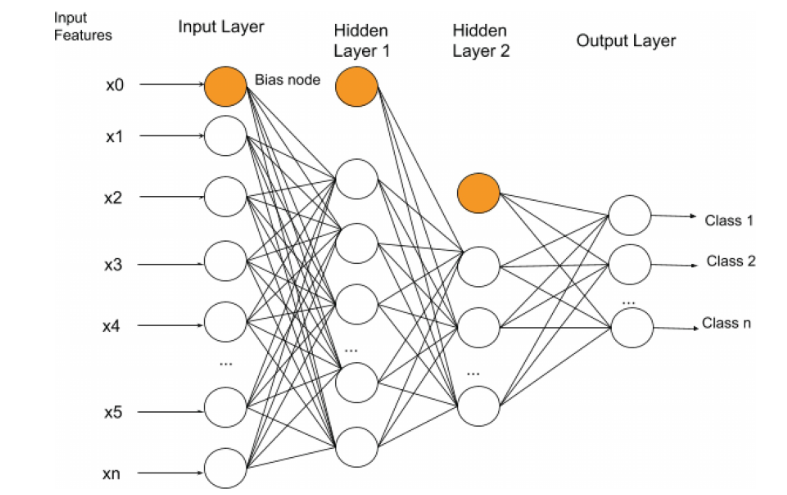
\includegraphics[width=0.8\linewidth]{tex/img/MLP.PNG}
        \caption{Multi layer perceptron \cite{ansari2020building}}
        \label{fig:MLP}
    \end{figure}
also known as the backpropagation algorithm, which executes in two stages as follows:
    \begin{itemize}
        \item \textbf{Forward Stage:} Activation functions start from the input layer in the forward stage and terminate at the output layer.
        \item \textbf{Backward Stage:} In the backward stage, weight and bias values are modified as per the model's requirements. In this stage, the error between the actual output and demand originates at the output layer and propagates backward to the input layer.
    \end{itemize}
A multi-layer perceptron model is a type of artificial neural network that has greater processing power and is capable of processing both linear and non-linear patterns. It is also capable of implementing logic gates such as AND, OR, XOR, NAND, NOT, XNOR, and NOR.

This model has multiple artificial neural networks with several layers, where the activation function is not linear as in a single-layer perceptron model. Instead, it can be executed with various activation functions such as sigmoid, TanH, ReLU, etc., for deployment. \cite{ansari2020building}, \cite{nielsen2015neural}
\end{enumerate}

\subsection{Deep Learning}
Deep learning is a type of artificial neural network or multilayer perceptron. It is a subset of machine learning that focuses on using artificial neural networks and representational learning. The term "deep" in deep learning refers to the use of multiple layers in the network. These methods can be supervised, semi-supervised, or unsupervised. \cite{vargas2017deep}

Various deep-learning architectures, such as deep neural networks, deep belief networks, deep reinforcement learning, recurrent neural networks, convolutional neural networks, and transformers, have been successfully applied to several fields, including computer vision, voice recognition, signal processing, natural language processing (NLP), machine translation, bio-informatics, drug or medical purposes, climate forecasting, material inspection, and board game programs. These architectures have produced remarkable results that are comparable to, and in some cases, surpassing human expert performance. \cite{hosseini2020deep}

\subsubsection{Deep Learning or Multilayer Perceptron Architecture}
A multilayer perceptron consists of at least three types of layers: the input layer, the hidden layers, and the output layer. You can have more than one hidden layer. Each layer contains one or more neurons. A neuron performs some computation on the inputs it gets and generates outputs. The output from the neurons is sent as input to the next layer, except in the case of the output layer.

\begin{enumerate}
    \item \textbf{Input layer: } This is the primary component of Perceptron, which accepts the initial data into the system for further processing. Every input node in the system holds a numerical value that is real and can be expressed as a number.
In a neural network, the input layer receives raw input data like image, text, etc. It then passes it on to the next layer. Each node in the input layer represents a feature or an attribute of the input data. These nodes act as receptors for the raw input information and are connected to the nodes in the next layer, which is typically a hidden layer.
    
Here are some key points about the input layer:
    \begin{enumerate}
\item Nodes/Neurons: The nodes in the input layer are also called input neurons. Each neuron corresponds to a specific feature or dimension of the input data.
\item Input Features: If you're working with a dataset of, for example, images, each node in the input layer might represent a pixel's intensity or color values. In the case of text data, each node could represent a unique word or a character.
\item No Processing: The nodes in the input layer do not perform any processing on the input data. They simply pass the raw input values to the next layer. The actual computation and learning occur in the subsequent layers, particularly in the hidden layers.
\item Connections: Each node in the input layer is connected to every node in the next layer (usually a hidden layer) through weights. These weights determine the strength of the connection between nodes and play a crucial role in the learning process of the neural network.
    \end{enumerate}
    The input layer of a neural network consists of neurons that are equal in number to the features of the data. Along with these neurons, additional nodes called bias nodes can also be included in each layer. The primary purpose of the bias node is to provide control over the output of the layer. Although not strictly necessary in deep learning, it is still a common practice to add a bias node.
    
    \textbf{Total Number of Neurons in the input layer} = The number of input features without a bias = (The number of input features + 1) with a bias 
    \cite{ansari2020building}\\
    \item \textbf{Hidden Layers: } Hidden layers in a neural network refer to the layers that come between the input layer and the output layer. They are called "hidden" because their outputs are not directly observable or part of the final network output during the training phase. At least one hidden layer is necessary for a neural network to function as this is where the learning occurs. The neurons in this layer perform the computations required for learning. Generally, for most cases, a single hidden layer is sufficient for learning. However, as required to model real-world situations, the number of hidden layers can be increased. As the number of hidden layers increases, the computation complexity of the network also increases, which leads to an increase in computation time.
    \\
    
    \textbf{Total Number of Neurons in the hidden layer} = A common practice is to take two-thirds (or 66 percent) of the number of neurons in the previous layer.\\
    
    For example, if the number of neurons in the input layer is 100, the number of neurons in the first hidden layer will be 66 and in the next hidden layer will be 43, and so on. Again, there is no magic number, and you should tune the neuron counts based on the model accuracy.
    \item \textbf{Output Layer: } The output layer is the final layer in a neural network, responsible for producing the model's predictions or outputs based on the learned representations from the preceding layers. The number of neurons in the output layer depends on the problem type that the neural network is supposed to solve. \\
    \textbf{Nodes in the Output Layer can be used for:}
    \begin{itemize}
        \item \textbf{For binary classification: } there is typically one node with a sigmoid activation function, producing a probability output.\\
        \item \textbf{For multi-class classification: } when the network has to predict one of many classes, the output layer has as many neurons as the number of all possible classes.\\
        \item \textbf{For regression tasks: } there is usually a single node with a linear activation function, producing a continuous output/ when the network has to predict a continuous value, such as the closing price of stocks, the output node has only one neuron. \cite{calin2020deep}, \cite{nielsen2015neural}
    \end{itemize}
\end{enumerate}
\subsubsection{Forward propagation}

A feedforward neural network is a type of artificial neural network comprising neurons interconnected in a manner that avoids cyclic connections. This architecture represents the most basic form of the neural network, where data propagation occurs unidirectionally, from the input layer through the hidden layer(s), and ultimately to the output layer. Unlike its counterparts, this network lacks any loopback or feedback mechanism, enabling a linear flow of information through its layers. \cite{coates2011analysis} \cite{ansari2020building} 
\begin{figure}[H]
    \centering
    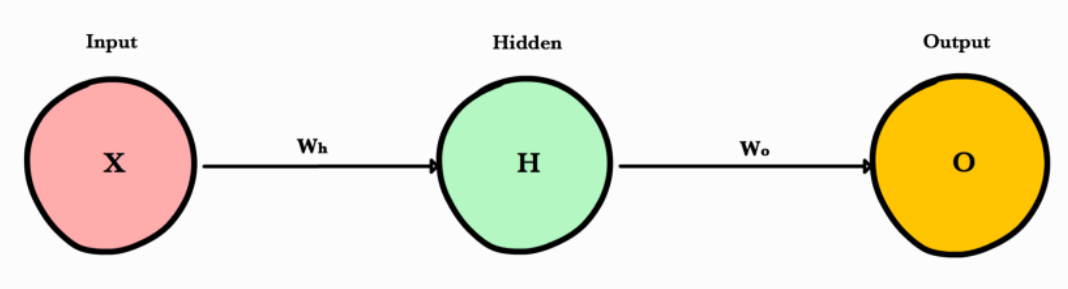
\includegraphics[width=0.7\linewidth]{tex/img/Forwardpropagation.PNG}
    \caption{Forward Propagation \cite{ajitjaokar}}
    \label{fig:enter-label}
\end{figure}
a single pass of forward propagation translates mathematically to:
\[Prediction=A(A(XW_{h})W_{o})\]
Where A:    is an activation function like ReLU, X is the input and $W_{h}$ and $W_{o}$ are weights.\\

\textbf{Steps}\\
- Calculate the weighted input to the hidden layer by multiplying X by the hidden weight $W_{h}$.\\
- Apply the activation function and pass the result to the final layer \\
- Repeat step 2 except this time X is replaced by the hidden layer’s output, H \cite{ansari2020building}, \cite{nielsen2015neural}

\subsubsection{BackPropagation: }
The main objective of back propagation is to modify or adjust the weights in the neural network in a way that corresponds to their contribution to the overall error. By consistently reducing the error associated with each weight, we can eventually obtain a set of weights that generate accurate predictions. \\
Here are the final 3 equations that together form the foundation of backpropagation. \cite{hecht1992theory} \cite{nielsen2015neural}
 \[
 Output Layer Error    E_{o} = (O-y).R'(Z_{o})
 \]
 \[ 
 Hidden Layer Error    E_{h} = E_{o}.W_{o}.R'(Z_{h})
 \]
 \[ 
 Cost-Weights Deriv \hspace{3mm}   LayerError.LayerInputs
 \]


\begin{figure}[H]
    \centering
    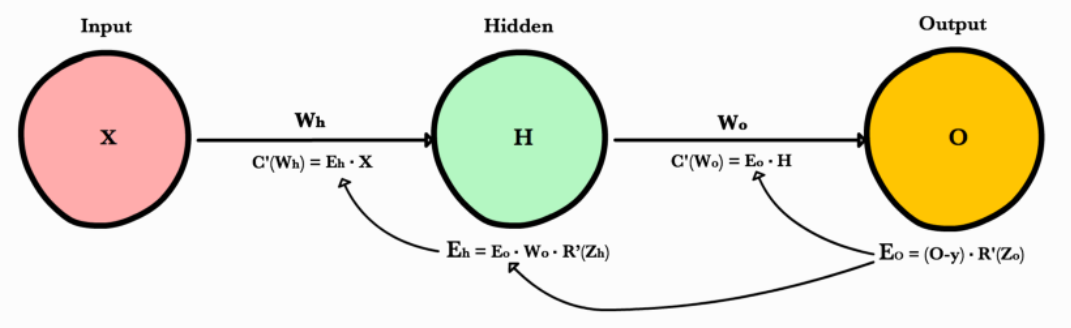
\includegraphics[width=0.8\linewidth]{tex/img/backward_propagation.PNG}
    \caption{Backward Propagation \cite{ajitjaokar}}
    \label{fig:backward_propagation}
\end{figure}
\subsubsection{Activation function}
The activation function plays a crucial role in determining whether a neuron should be activated (turned on or off) based on whether its input is relevant for model prediction. This function normalizes the output of each neuron to a range between 0 and 1 or between -1 and 1. Different mathematical functions are utilized as activation functions for various purposes.\cite{sharma2017activation}, \cite{apicella2021survey}, \cite{bfortuner_mlglossary}

we can broadly divide the activation function into two: \\
\begin{itemize}
    \item \textbf{Linear Activation Function: } Commonly used in the output layer for regression tasks where a continuous range of values is desired. A linear activation function computes a weighted sum of its input without introducing non-linearity, and The output is a linear transformation of the input. 
    \begin{figure}[H]
        \centering
        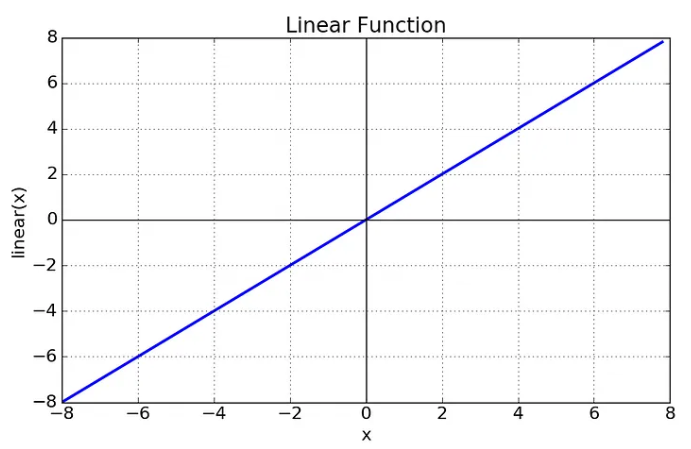
\includegraphics[width=0.5\linewidth]{tex/img/Linear_function.PNG}
        \caption{Linear Activation Function}
        \label{fig:LAF}
    \end{figure}
    \textbf{Equation: }
    \(f(x)=cx\) \\where c is constant.\\
    
    The output of the linear activation function varies from $-\infty$ to  $+\infty$, as shown in Figure above.
     If you choose to use a linear activation function, the last layer of your neural network will simply be a linear function of the first layer, regardless of how many layers the network has. This means that your network can only learn linear dependencies between the input and output, which is insufficient for solving complex problems like computer vision. Therefore, using a linear activation function is not recommended for such problems. \cite{bfortuner_mlglossary}\\
     \item \textbf{Non-linear Activation Function: } A non-linear activation function introduces non-linearity into the network, enabling it to learn complex relationships and representations. It facilitates the model's ability to generalize and differentiate outputs with diverse data.
    \begin{figure}[H]
        \centering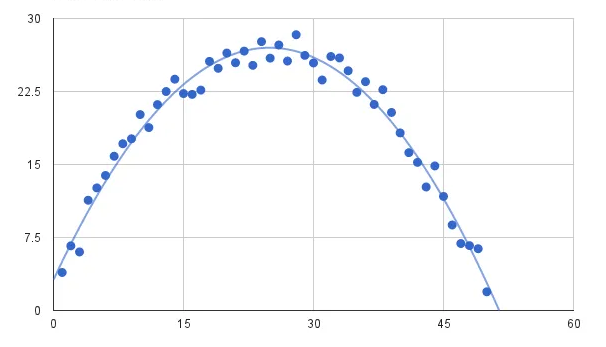
\includegraphics[width=0.5\textwidth]{Non-Linear.PNG}
        \caption{Non-Linear Activation Function}
    \end{figure}
    Essential for training deep neural networks as it allows the network to capture complex patterns and relationships in the data, They allow the network to capture intricate relationships between features, which is crucial for tasks like image recognition, natural language processing, and more.
    \begin{enumerate}
        \item \textbf{Sigmoid or Logistic Activation Function: } 
    The sigmoid activation function calculates the neuron output using the sigmoid function, as shown here:
    $$\phi(z)=\frac{1}{1+e^{-z}}$$
    \begin{figure}[H]
        \centering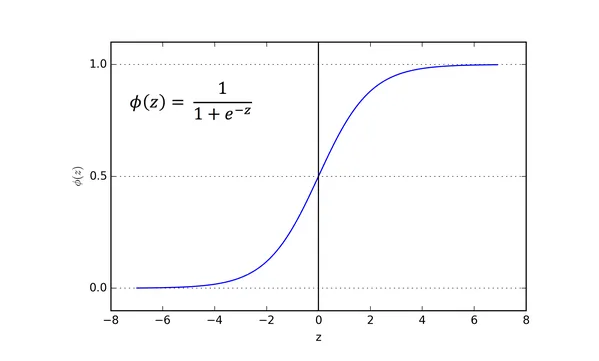
\includegraphics[width=0.5\textwidth]{sigmoid_Activation.PNG}
        \caption{Sigmoid Activation Functioin}
    \end{figure}
    where \(z\) is calculated like \\
    
    $$z=X_0+\sum_{i=0}^{i=n}w_{i}x_{i}$$
    
    The sigmoid function is a mathematical operation that always yields a value between 0 and 1. This makes the output spontaneous, without many overrides as the input value fluctuates. Additionally, the sigmoid function is very useful as it does not generate a constant value from the first-order derivatives because it is a non-linear function.
    
    The sigmoid function is a mathematical function that always produces an output value between 0 and 1. This characteristic results in a smooth output without many jumps as the input value fluctuates. Another benefit of the sigmoid function is that it is nonlinear, and its first-order derivative does not generate a constant value.
    \item \textbf{Tanh or hyperbolic tangent Activation Function}
    
    The Tanh function is a type of activation function, commonly used in neural networks. Its behavior is similar to the sigmoid activation function, but with some notable differences. The Tanh function is zero-centered, and The range of the tanh function is from (-1 to 1).
    
    \begin{figure}[H]
        \centering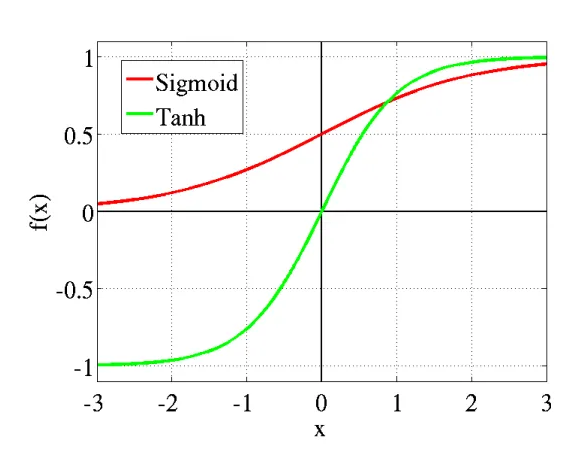
\includegraphics[width=0.5\textwidth]{Tangent_activation.PNG}
        \caption{Tangent Activation Functioin}
    \end{figure}
    
    The TanH activation function calculates the neuron output using:\\
    $$tanh(z)=\frac{e^{z}-e^{-z}}{e^{z}+e^{-z}}$$
    The TanH is useful when it comes to mapping the values; the negative inputs will be mapped strongly to negative, and the same for positive inputs too, and the zero inputs will be mapped near zero.
    \item \textbf{ReLU (Rectified Linear Unit) Activation Function}
   The Rectified Linear Unit (ReLU) is a widely used activation function in deep learning, particularly for computer vision tasks. ReLU is preferred for image processing because it can handle non-negative values, which is a common characteristic of image pixels. One of the key advantages of ReLU is its computational efficiency, which makes it suitable for large-scale models. Furthermore, ReLU is a nonlinear function with a derivative, allowing for backpropagation and weight adjustment during training. This property is essential for the neural network to learn from the data and improve its performance over time.
    
    \begin{figure}[H]
        \centering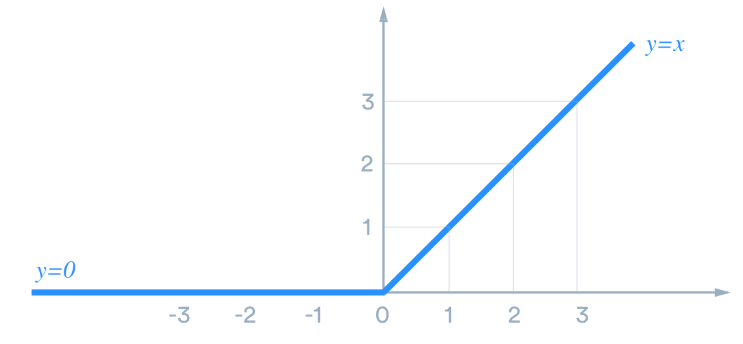
\includegraphics[width=0.5\textwidth]{Relu_Activation.PNG}
        \caption{ReLU Activation Functioin}
    \end{figure}
    
    
    $$f(x)=max(0,x)$$
    it ranges from 0 to +$\infty$\\
    \item  \textbf{Leaky ReLU Activation Function}
    The leaky rectified linear unit (ReLU) is a widely used activation function in deep learning models. The function introduces a small negative slope in the negative region, which allows for backpropagation for negative inputs, thereby avoiding the vanishing gradient problem. However, a drawback of this function is that it produces inconsistent outputs for negative values. This is because the negative slope of the activation function results in a non-zero output for negative inputs, which is not consistent with the expected behavior of an activation function. Nonetheless, the leaky ReLU remains a popular choice for deep neural networks due to its ability to improve the training of deep models.
    \begin{figure}[H]
        \centering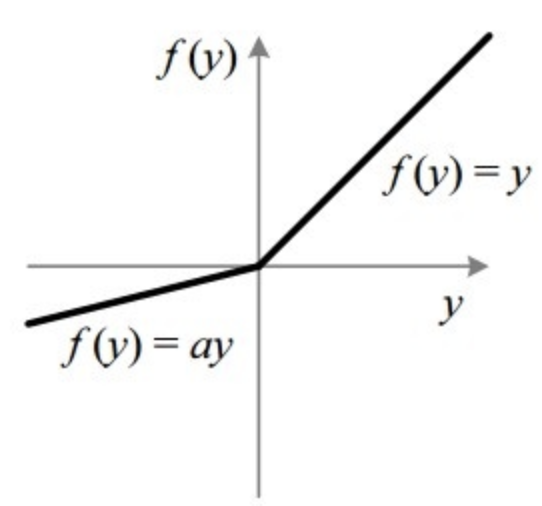
\includegraphics[width=0.5\textwidth]{leaky_relu.png}
        \caption{Leaky ReLU Activation Functioin}
    \end{figure}
    
    $f(y)=\left\{\begin{array}{rcl}
         \alpha y & \mbox{for} & y<0\\
         y & \mbox{for} & y\geq 0
    \end{array}\right.$\\
    \item \textbf{SELU Actiovation Function}
    A scaled exponential linear unit (SELU) computes neuron outputs using the following equation:
    
    $f(\alpha,x)=\lambda\left\{\begin{array}{rcl}
         \alpha (e^{x}-1) & \mbox{for} & x<0\\
          x & \mbox{for} & x\geq 0
    \end{array}\right.$\\
    \\
    where the value of $\lambda$ = 1.05070098 and the value of $\alpha$ = 1.67326324. These values are fixed and do not change during backpropagation.[Orielly]
    \begin{figure}[H]
        \centering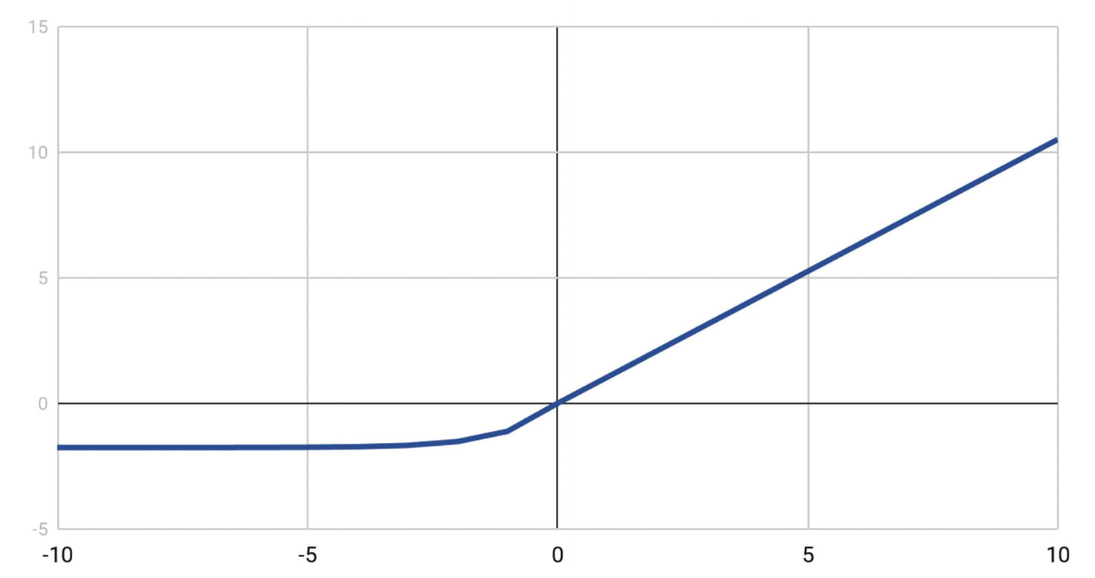
\includegraphics[width=0.5\textwidth]{SELU_activation.PNG}
        \caption{SELU Activation Functioin}
    \end{figure}
    
   SELU is an activation function that has the property of self-normalization. This means that with SELU, the entire network is self-normalizing, which makes it efficient in terms of computation and helps it converge faster. Additionally, SELU overcomes the issues of exploding or vanishing gradients that occur when the input features are too high or too low.
    \item \textbf{Softplus Activation Function}
    The softplus activation function applies smoothing to the activation function value 
    \(z\) . It uses the log of exponent as follows:\\
    
    $$f(x)=lon(1+e^{z})$$\\
    \\
    Softplus is also called the SmoothReLU function. The first derivation of the softplus function is  $\frac{1}{1+e^{z}}$, which is the same as the sigmoid activation function. 
    
    \begin{figure}[H]
        \centering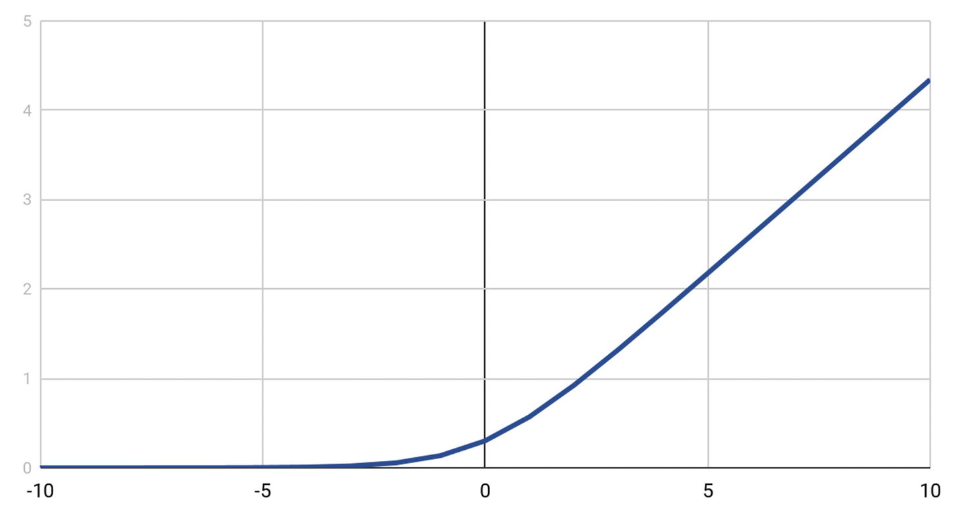
\includegraphics[width=0.5\textwidth]{Softplus_activation.PNG}
        \caption{Softplus Activation Function}
    \end{figure}
    \item \textbf{Softmax}
    The Softmax function operates on a vector of real numbers by normalizing it to create a probability distribution that generates outputs between 0 and 1. The resulting probabilities have the property that the sum of all output values is equal to 1. This function is typically utilized as the activation function for the output layer of a classification neural network. The interpreted output values represent prediction probabilities for each class.
    \begin{figure}[H]
        \centering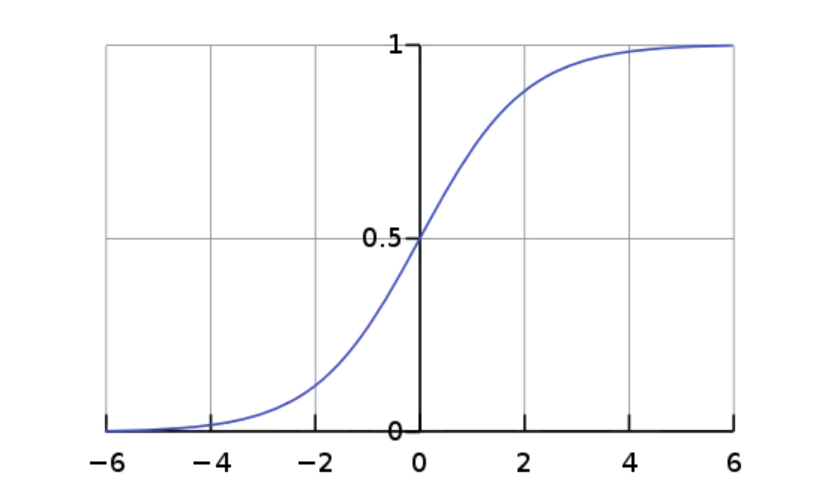
\includegraphics[width=0.5\textwidth]{Softmax.PNG}
        \caption{Softmax Activation Function}
    \end{figure}
    $$\sigma(z)_{i}=\frac{e^{z_{i}}}{\sum_{j=1}^{k}e^{z_{j}}}$$ for \(i\)=1,...., k and z=$(z_{1}....,z_{k})$ $\epsilon R^{k}$
    \end{enumerate}
\end{itemize}

\subsubsection{Loss Function/Error Function}
A loss function is a function that measures how well a neural network models the training data by comparing the target and predicted output values. During training, the goal is to minimize the loss between the predicted and target outputs.
The equation of error may be written in a simplified form as follows:\\

\(Error = Expected outcome - Predicted outcome\)\\

When a neural network begins the learning process, it initializes weights and calculates output from each neuron using an activation function. It then computes the error, adjusts the weights, recalculates outputs, and re-evaluates errors, until it reaches the minimum error. The weights that give the minimum errors are considered the final weights and the network is considered "learned" at this stage.

In calculus, if the first derivative of a function is zero, then the function at that point is either a minimum or a maximum. The neural network training process aims to find the minimum point where the first derivative is zero. To achieve this, a neural network must have an \textbf{error function} that calculates the first derivative and identifies the points (weights and biases) where the error function is minimum. The type of error function used depends on the type of model being trained. These error functions are also called loss functions or simply losses.\\

The error functions are broadly divided into the following three categories: \cite{ansari2020building}, \cite{heaton2018ian}\\
\begin{itemize}
    \item \textbf{Regression loss functions} are used when we want to train models to predict continuous value outcomes, typically a numerical value. To measure the difference between the predicted and actual target values, different loss functions are employed. The following are some widely used regression loss functions:\\
    \begin{itemize}
    \item \textbf{Mean Squared Error (MSE) Loss:} This is the default error function for regression problems. This is the preferred loss function if the distribution of the target variable is normal or Gaussian. This function has numerous properties that make it especially suited for calculating loss. The difference is squared, which means it does not matter whether the predicted value is above or below the target value; however, values with a large error are penalized.\\
    $$MSE=\frac{1}{n}\sum_{i=1}^{n}(y^{(i)}-\hat{y}^{(i)})^{2}$$
    \item  \textbf{Mean Absolute Error (MAE) Loss:}  MAE finds the average of the absolute differences between the target and the predicted outputs.
    $$MAE=\frac{1}{n}\sum_{i=1}^{n}|y^{(i)}-\hat{y}^{(i)}|$$
    In some cases, this loss function serves as an alternative to MSE. As mentioned earlier, MSE is highly sensitive to outliers, which can significantly affect the loss due to the squared distance. To mitigate this, MAE is used when the training data has a substantial number of outliers.
    \item \textbf{The Mean Squared Logarithmic Error (MSLE)} The Mean Squared Logarithmic Error (MSLE) is a loss function that is commonly used in regression tasks. It is particularly useful when the target values span multiple orders of magnitude. MSLE measures the mean squared difference between the natural logarithm of the predicted values and the natural logarithm of the true values. This can be especially helpful when there is a wide variation in the scale of the target values.
    The formula for MSLE is as follows:
     $$MSLE(y,\hat{y})=\frac{1}{n}\sum_{i=1}^{n}(log(1+y^{(i))}-log(1+\hat{y}^{(i)}))^{2}$$
     where: \\
     $y^{i}: $ is the true target value for the \(i\)-th sample.\\
     $\hat{y}^{(i)}: $ is the predicted target value for the \(i\)-th sample.
     \item \textbf{Huber Loss: } The Huber loss, also referred to as the smooth L1 loss, is a commonly used loss function in regression tasks. It is designed to be less sensitive to outliers compared to the Mean Squared Error (MSE) loss function while retaining the benefits of a quadratic loss function for smaller errors.

     $$Huber(y,\hat{y})=\frac{1}{n}\sum_{i=1}^{n}L_{\delta}(y^{(i))}-\hat{y}^{(i)})$$
     where: \\
     $y_{i}: $ is the true target value for the \(i\)-th sample.\\
      $y^{i}: $ is the predicted target value for the \(i\)-th sample.\\
      $n: $ is the total number of samples.\\
      $L_{\delta}(x)$ is defined as:
      
      $L_{\delta}(x)=\left\{\begin{array}{rcl}
           \frac{1}{2}x^{2} & \mbox{for} & |x| \leq \delta \\
          \delta(|x|-\frac{1}{2}\delta) & otherwise 
      \end{array}\right.$\\
      \textbf{Benefit: } One big When training neural networks, using Mean Absolute Error (MAE) can cause a problem due to its large gradient, which can result in missing the minima at the end of training when using gradient descent. In contrast, as the loss gets closer to its minima, the gradient decreases when using Mean Squared Error (MSE), making it more accurate.
    
    To address this issue, Huber loss can be very useful since it curves around the minima, decreasing the gradient. Additionally, Huber loss is more resistant to outliers than MSE. Therefore, it combines the desirable properties of both MSE and MAE.
    \item  \textbf{Log-Cosh loss: } The Log-Cosh loss is a smooth and differentiable approximation of the Huber loss, often used in regression tasks. Similar to the Huber loss, it aims to be less sensitive to outliers than the Mean Squared Error (MSE) loss, but it has the advantage of being continuously differentiable.
     $$Log-Cosh(y,\hat{y})=\frac{1}{n}\sum_{i=1}^{n}Log(cosh(y^{(i))}-\hat{y}^{(i)}))$$
     where: \\
      $y_{i}: $ is the true target value for the \(i\)-th sample.\\
      $y^{i}: $ is the predicted target value for the \(i\)-th sample.\\
      $n: $ is the total number of samples.\\
      \(Cosh: \) is the hyperbolic cosine function.\\
      The optimization goal during training is to minimize the Log-Cosh loss, and the model adjusts its parameters to achieve predictions that result in smaller Log-Cosh loss values. The Log-Cosh loss is often considered when a balance between the robustness of the Huber loss and the differentiability of the MSE loss is desired.
      \item \textbf{Quantile loss function: } Quantile loss is a loss function used in quantile regression, where the goal is to predict not just a central tendency (like the mean in traditional regression) but rather different quantiles of the target distribution. It is particularly useful when you want to estimate a range of possible values for a prediction.
      $$L_{\gamma}(y, y^{p})=\sum_{i=y_{i}<y_{i}^{p}}(\gamma-1).|y_{i}-{y_{i}^{p}}|+ \sum_{i=y_{i}\geq y_{i}^{p}}(\gamma).|y_{i}-y_{i}^{p}|$$

      The optimization goal during training is to minimize the Quantile Loss, and the model adjusts its parameters to achieve predictions that capture the desired quantiles of the target distribution. Quantile regression is particularly useful in scenarios where understanding the variability or uncertainty in predictions is essential.
      
    
     
    \end{itemize}
    \item \textbf{Binary classification loss functions} are used when we want to train models to predict a maximum of two classes (usually denoted as 0 and 1) and the true binary label, such as to compare and contrast different classes together. \\
          \begin{itemize}
          \item \textbf{Binary Crossentropy Loss (Log Loss): } The Binary Crossentropy Loss (Log Loss) is the default loss function for binary classification problems and is considered better than other functions. It calculates a score that reflects the average difference between the actual and predicted probability distributions for predicting class 1. This score is minimized, and a perfect cross-entropy value is set to 0. The function can only be used when the target value is within the range of (0,1).
          $$Binary Crossentropy(y, \hat{y})=\frac{1}{n}\sum_{i=1}^{n}[y_{i}log(\hat{y_{i}})+(1-y_{i})log(1-\hat{y_{i}})]$$

          It measures the cross-entropy between the true binary labels and the predicted probabilities. It penalizes deviations from the true labels by assigning higher penalties to confidently wrong predictions.
          \item \textbf{Hinge Loss (SVM Loss):} This is used mainly in support of vector machine–based binary classification and can be used when the target variable is in the range (-1, 1).
          $$Hinge-Loss(y,\hat{y})= \frac{1}{n}\sum_{i=1}^{n}max(0,1-y_{i}.\hat{y_{i}})$$

          Penalizes misclassifications linearly and encourages correct predictions to have a margin of at least 1.

          \item \textbf{Squared Hinge Loss: } The squared hinge loss function computes the squared value of the score hinge loss. This mathematical operation smooths the surface of the error function, rendering it numerically more tractable.
          \[
          \text{Squared Hinge Loss}(y,\hat{y})=\frac{1}{n}\sum_{i=1}^{n}max(0,1-y_{i}.\hat{y_{i}})^{2}
          \]
      \end{itemize}
    \item \textbf{Multiclass classification loss functions} are used when our models need to predict more than two classes/are used to measure the difference between predicted class probabilities and true class labels in scenarios where there are more than two classes, such as object detection. \\
          \begin{itemize}
          \item \textbf{Categorical Crossentropy Loss: } used for multiclass classification tasks with one-hot encoded true class labels. It is used to measure the cross-entropy between the true distribution and the predicted class probabilities.
          $$Categorical Crossentropy(y,\hat{y_{i}})=-\frac{1}{n}\sum_{i=1}^{n}\sum_{j=1}^{m}y_{ij}log(\hat{y_{ij}})$$
          \item \textbf{Sparse Categorical Crossentropy Loss: } Similar to categorical crossentropy but used when true class labels are provided as integers rather than one-hot encoded vectors.
          $$Sparse Categorical Crossentropy(y,\hat{y})=-\frac{1}{n}\sum_{i=1}^{n}log(\hat{y_{i}[y_{i}]})$$
          Sparse cross-entropy performs the same cross-entropy calculation of error without requiring that the target variable be one hot-encoded before training and is used When you have a large number of classes in the target, for example, predicting dictionary words.
          \item \textbf{Kullback-Leibler divergence (KLD) loss: }The Kullback-Leibler divergence (KLD) loss is a measure of the dissimilarity between one probability distribution and a reference baseline distribution. A value of 0 for the KL divergence loss indicates that both distributions are identical. This statistical metric quantifies the amount of information loss, expressed in bits, when the predicted probability distribution is employed to approximate the target probability distribution.

        The KLD loss is a valuable tool for addressing complex problems, such as auto-encoders, which are utilized for learning high-dimensional representations. In the context of multiclass classification, KLD serves as a multiclass cross-entropy measure.
        \[
        \text{KL Divergence}(P \parallel Q) = \sum_{i \in \chi} P(i) \log\left(\frac{P(i)}{Q(i)}\right)
        \]
        where:\\
        For discrete probability distributions, P and Q are defined on the same sample space, $\chi$, the relative entropy from Q to P.
        \item \textbf{Cross-Entropy Loss (Sigmoid Crossentropy for Multilabel Classification): }
        Suitable for multilabel classification where each sample can belong to multiple classes. It measures the crossentropy for each class independently.

         \[
         \text{Cross Entropy Loss}(y,\hat{y})=-\frac{1}{n}\sum_{i=1}^{n}[y_{i}log(\sigma(\hat{y_{i}}))+(1-y_{i})log(1-\sigma(\hat{y_{i}}))]
         \]
      \end{itemize}

\end{itemize}

\subsubsection{Layers}
In a neural network, layers are the building blocks that organize and structure the computation. Each layer contains a group of nodes, or neurons, that process information.
\begin{itemize}
    \item \textbf{Convolutional Layer: } In convolutional neural networks (CNN), the convolution layer performs a linear operation by multiplying the input with a weight (kernel or filter), and it plays a critical role in the network. The layer comprises two primary components: \\
    \begin{itemize}
        \item \textbf{Kernel (Filter): } A convolution layer can comprise more than one filter. The size of the filter should be smaller than the input dimension intentionally, as it allows the filter to be applied at different positions on the input. Filters are useful for identifying significant features in a given input. By applying more than one filter to the same input, different features can be extracted. The output from multiplying the filter with the input creates a dimensional array called the "feature map."

        The Stride property controls the movement of the filter over the input. When the value is set to 1, the filter moves one column at a time over the input. When set to 2, the filter jumps two columns at a time as it moves over the input.
    \end{itemize}
    \item \textbf{Dropout Layer: } A dropout layer is a type of layer commonly used in neural networks to prevent overfitting. It takes the output of the previous layer's activations and randomly sets a certain fraction, known as the dropout rate, of the activations to 0. This effectively cancels or "drops out" those activations, helping to prevent the network from becoming too reliant on any one feature or pattern. The dropout rate is a tunable hyperparameter that can be adjusted to measure performance with different values. Typically, it is set between 0.2 and 0.5, but it can be set arbitrarily depending on the specific application and dataset.
    
    Dropout is a technique used during training of neural networks. During training, some of the activations in a layer are randomly dropped or turned off. However, at test time, no activations are dropped, instead, they are scaled down by a factor of the dropout rate. This is to account for the fact that more units are active during test time than during training time. The idea behind dropout is to introduce some noise into the layer in order to disrupt any interdependent learning or coincidental patterns that may occur between units in the layer that are not significant. This helps to prevent overfitting and improve the generalization performance of the network. \\
    \item \textbf{Pooling layer: }Pooling layers often take convolution layers as input. A complicated dataset with many objects will require a large number of filters, each responsible for finding patterns in an image so the dimensionally of a convolutional layer can get large. It will cause an increase in parameters, which can lead to over-fitting. Pooling layers are a type of technique that is used to reduce the dimensionality of high-dimensional data. Similar to convolutional layers, pooling layers also have a kernel size and stride. The kernel size is typically smaller than the feature map, with a standard size of 2x2 and a stride of 2. There are two main types of pooling layers that are commonly used.

    The first type is the max pooling layer. The Max pooling layer will take a stack of feature maps (convolution layer) as input. The value of each node in the max pooling layer is calculated by taking the maximum value of the pixels contained in a sliding window. This operation helps to reduce the size of the feature maps while preserving the most important information.
    
    The other type of pooling layer is the: \\
    \textbf{Average Pooling layer}. The average pooling layer calculates the average of pixels contained in the window. It's not used often but you may see this used in applications for which smoothing an image is preferable.\\
    \item \textbf{Fully-connected/Linear Layer: } A fully-connected layer, also called a linear layer, is a type of layer in a neural network where all the inputs from one layer are connected to every activation unit of the next layer. Usually, the last few layers in machine learning models are fully-connected ones, which output a class prediction based on the features learned in the previous layers.

To input a vector of nodes activated in the previous convolutional layers, the fully-connected layer passes it through one or more dense layers before sending it to the output layer. An activation function is used to make a prediction before the vector reaches the output layer. While the convolutional and pooling layers tend to use a ReLU function, the fully-connected layer can use two activation functions depending on the classification problem:

- Sigmoid:  is a mathematical function that is commonly used for binary classification problems. It is a logistic function that has a characteristic "S" shaped curve.
- Softmax: A more generalized logistic activation function that ensures the values in the output layer sum up to 1. It is commonly used for multi-class classification.

The activation function outputs a vector with the same dimensions as the number of classes to be predicted. The output vector yields a probability between 1 and 0 for each class. \cite{schmidhuber2015deep}, \cite{goodfellow2016deep}\\
   
\subsubsection{Optimizer}
An optimizer is an algorithm or method used to adjust the parameters of the neural network (weights and biases) during the training process. The primary goal of an optimizer is to minimize the loss function, which measures the difference between the predicted output and the true target values.

During training, the neural network makes predictions, and the optimizer adjusts the model's parameters based on the error (loss) between these predictions and the actual target values. The optimization process involves finding the optimal set of parameters that minimize the loss, enabling the neural network to make accurate predictions on unseen data. \cite{choi2019empirical}, \cite{ansari2020building} 

Some commonly used optimizers in neural networks include:
\begin{itemize}
    \item \textbf{Adaptive gradient (Adagrad): } Adaptive gradient (Adagrad) is a technique that adjusts the learning rate according to a specific parameter. 
\begin{itemize}
    \item This method ensures that parameters with higher gradients or frequent updates have a slower learning rate, so as not to overshoot the minimum value.
    \item parameters with low gradients or infrequent updates have a faster learning rate, allowing them to be trained quickly.
    \item  It divides the learning rate by the sum of squares of all previous gradients of the parameter.
    \item When the sum of the squared past gradients has a high value, it basically divides the learning rate by a high value, so the learning rate will become less.
    \item Similarly, if the sum of the squared past gradients has a low value, it divides the learning rate by a lower value, so the learning rate value will become high.
    \item This implies that the learning rate is inversely proportional to the sum of the squares of all the previous gradients of the parameter.
    \end{itemize}
    \[
    g_{t}^{i}=\frac{\partial J(w_{t}^{i})}{\partial \mathbf{W}}
    \]
    \[
    \mathbf{W}=\mathbf{W}-\alpha\frac{\partial J(\omega_{t}^{t})}{\sqrt{\sum_{r=1}^{t}(g_{r}^{i})^2+\epsilon}}
    \]
    where: \\
     $g_{t}^{i}$  the gradient of a parameter\\
    $\alpha$ : the learning rate\\
    $\epsilon: $ very small value to avoid dividing by zero
    
    \item \textbf{Adaptive delta(Adadelta): } Adadelta is a type of stochastic gradient descent algorithm that offers adaptive techniques for hyperparameter tuning. The name Adadelta is derived from "adaptive delta", where delta refers to the difference between the current weight and the newly updated weight.

    Adadelta is an improved version of Adagrad that adjusts learning rates based on a moving window of gradient updates, instead of accumulating all past gradients. This allows Adadelta to continue learning even after many updates have been made.
    
    The update rule in Adadelta eliminates the need to set a default learning rate, making it unnecessary to specify a learning rate.
    
    \[
    v_{t}=\rho v_{t-1}+(1-\rho)\bigtriangledown_{\theta}^{2}J(\theta)
    \]
    \[
    \bigtriangleup\theta=\frac{\sqrt{\omega_{t}+\epsilon}}{\sqrt{v_{t}+\epsilon}}\bigtriangledown_{\theta}J(\theta)
    \]
    \[
    \theta=\theta-\eta\bigtriangleup\theta
    \]
    $\omega_{t}=\rho\omega_{t-1} + (1-\rho)\bigtriangleup\theta^{2}$
    \item \textbf{Adam Optimizer: } The Adam optimizer combines concepts from both RMSProp and Momentum to help in computing adaptive learning rates for each parameter. It works as follows:
    \begin{itemize}
        \item Firstly, it computes the exponentially weighted average of past gradients $(v_{dW})$
        \item  Secondly, it calculates the exponentially weighted average of the squares of past gradients $(s_{dW})$
        \item Thirdly, to counteract any bias towards zero, a bias correction is applied to these averages  $(v_{dW}^{corrected}, s_{dW}^{corrected})$
        \item Lastly, the parameters are updated using the information from the calculated averages\\
        \[v_{dW}=\beta_{1}v_{dW}+(1-\beta_{1})\frac{\partial J}{\partial W}\]
        \[
        s_{dW}=\beta_{2}s_{dW}+(1-\beta_{2}) \left(\frac{\partial J}{\partial W}\right)^{2}
        \]
        \[
         v_{dW}^{corrected}=\frac{v_{dW}}{1-(\beta_{1})^{t}}
        \]
        \[
         s_{dW}^{corrected}=\frac{s_{dW}}{1-(\beta_{1})^{t}}
        \]
        \[
        W=W-\alpha\frac{v_{dW}^{corrected}}{\sqrt{s_{dW}^{corrected}} + \epsilon}
        \]
        where:\\
        $v_{dW}$-  the exponentially weighted average of past gradients\\
        $s_{dW}$- the exponentially weighted average of past squares of gradients\\
        $\beta_{1}$- hyperparameter to be tuned\\
        $\beta_{2}$- hyperparameter to be tuned\\
        $\frac{\partial J}{\partial W}$ - cost gradient with respect to current layer\\
        W- the weight matrix (parameter to be updated)\\
        $\alpha$ - the learning rate\\
        $\epsilon$ - very small value to avoid dividing by zero\\
    \end{itemize}
    \item \textbf{RMSProp Optimizer: } RMSProp optimizer is an adaptive learning rate optimization algorithm that helps to speed up convergence. It does this by keeping an exponentially weighted average of past gradient squares and dividing the learning rate by this average. This process results in a more efficient and faster convergence of the algorithm.
    \[
    s_{dW} = \beta s_{dW} + (1-\beta)\left(\frac{\partial J}{\partial W}\right)^{2}
    \]
    \[
    W = W-\alpha\frac{\frac{\partial J}{\partial W}}{\sqrt{s_{dW}^{corrected}}+ \epsilon}
    \]
    
    where: \\
    s - the exponentially weighted average of past squares of gradients\\
    $\frac{\partial J}{\partial W}$-  cost gradient with respect to current layer weight tensor\\
    W - weight tensor\\
    $\beta$- hyperparameter to be tuned\\
    $\alpha$- the learning rate\\
    $\epsilon$- very small value to avoid dividing by zero.
    \item \textbf{Stochastic Gradient Descent(SGD) Optimizer: } Stochastic Gradient Descent (SGD) is a widely used optimization algorithm for training neural networks and other machine learning models. It is a variant of the gradient descent optimization algorithm that processes each training example individually rather than using the entire dataset in each iteration. This property makes it well-suited for large datasets. Optionally, partition the dataset into mini-batches of a fixed size.
    \begin{itemize}
        \item For each mini-batch or individual example:
        \item Compute the gradient of the loss with respect to the model parameters.
        \item Update the model parameters in the opposite direction of the gradient to minimize the loss.
    \end{itemize}.\\
    The update rule for the model parameters $\theta$ is given by:
    \[
    \theta_{t} = \theta_{t-1}-\alpha\bigtriangledown J(\theta_{t-1},x_{i}, y_{i})
    \]\\
    where: \\
    $\alpha : $  is the learning rate, a hyperparameter that controls the size of the steps taken during optimization.\\
    $\bigtriangledown J(\theta_{t-1},x_{i}, y_{i}$ is the gradient of the loss function $\mathbf{J}$ with respect to the parameters $\theta$ for the example $x_{i}, y_{i}$
\end{itemize}



\subsubsection{Regularization}
Regularization techniques are widely used in machine learning to reduce overfitting and improve the generalization performance of models. These methods introduce constraints or penalties to the training process, which encourage the model to be simpler and more robust. By doing so, they help to prevent the model from fitting too closely to the training data, thereby improving its ability to generalize to new, unseen data. \cite{goodfellow2016deep}, \cite{ansari2020building}, \cite{bishop2006pattern}
\begin{itemize}
    \item \textbf{Data Augmentation: }
    Having more data is the surest way to get better consistent estimators (ML model), in contrast having a small dataset will lead to the well-known problem of overfitting.
    Data augmentation refers to the technique of artificially increasing the size of a dataset by applying various transformations to the existing data. This is often used in deep learning, particularly in computer vision tasks, to improve the performance of neural networks.
    There are various types of data augmentation techniques, including:
    \begin{enumerate}
        \item  Flipping: horizontally or vertically flipping an image.
        \item Rotation: Rotating an image by a certain degree is the process of rotating the image based on a specific angle.
        \item Zooming: zooming in or out of an image.
        \item Translation: shifting an image horizontally or vertically.
        \item Cropping: cropping a portion of an image.
        \item Adding noise: adding random noise to an image.
        
    \end{enumerate}
    
    These techniques can be used individually or in combination to generate new data samples. By increasing the size of the dataset, the neural network is exposed to more variations of the same data, which helps improve its ability to generalize and make accurate predictions on new, unseen data. \cite{shorten2019survey}\\
    \item \textbf{Dropout: } is a technique used to reduce overfitting in neural networks. It works by randomly ignoring selected neurons during training, which prevents complex co-adaptations on the training data. 

    During the training process, some of the neurons are randomly dropped out, meaning that their contribution to the activation of downstream neurons is temporarily removed on the forward pass. Additionally, any weight updates are not applied to the neuron on the backward pass. 
    
    Simply put, the process of ignoring some of the neurons occurs during a particular forward or backward pass. The probability of randomly selecting nodes to be dropped out can be easily adjusted (e.g. 0.1\%) each weight update cycle.
    
    It is important to note that Dropout is only used during the training of a model and is not used when evaluating the model. \\
    \item \textbf{Early Stopping: } Early stopping is an alternative technique that can be used to prevent overfitting. This approach involves using the validation error to decide when to stop training the neural network.

    The biggest challenge in training a neural network is determining how long to train the model. If you train the model too little, it will result in underfitting in both the train and test sets. On the other hand, if you train it too much, it will overfit the training set and perform poorly on the test sets.
    
    The key is to train the network long enough that it can learn the mapping from inputs to outputs, but not so long that it overfits the training data. One possible solution is to treat the number of training epochs as a hyperparameter and train the model multiple times with different values. Then, you can select the number of epochs that results in the best accuracy on the train or a holdout test dataset.
    
    However, this solution requires training and discarding multiple models, which can be time-consuming and resource-intensive. \cite{goodfellow2016deep}\\
    \item \textbf{Ensembling: } Ensemble methods are machine-learning techniques that combine multiple models into one predictive model. There are two primary approaches to ensembling: Bagging and Boosting.:
    \begin{itemize}
        \item \textbf{Bagging} Bagging, which stands for bootstrap aggregation, is a technique that reduces the variance of an estimate by averaging multiple estimates. It involves training a large number of "strong" learners in parallel. A strong learner is a model that is relatively unconstrained. Bagging then combines all the strong learners to obtain a smoother and more accurate prediction.
        \item  \textbf{Boosting}
        Boosting is a family of algorithms that convert weak learners into strong learners. It involves a sequence of models, with each one focusing on learning from the mistakes of the previous model. The final result is a combination of all the weak learners, which results in a single strong learner.
        
        Bagging utilizes complex base models to “smooth out” their predictions, while boosting uses simple base models to "boost" their combined complexity.
    \end{itemize}
    Bagging uses complex base models and tries to “smooth out” their predictions, while boosting uses simple base models and tries to “boost” their aggregate complexity.\\
    \item \textbf{Injecting Noise: } Noise is a phenomenon commonly introduced to the inputs as a technique for dataset augmentation. In situations where the dataset is small, the neural network may tend to memorize the training dataset instead of learning the general mapping from the inputs to the outputs. In other words, the model may only memorize specific input examples and their respective outputs. To solve this problem and enhance the structure of the mapping, one approach is to add random noise to the inputs.

    By adding noise, the network becomes less prone to memorizing the training samples since they keep changing all the time. This leads to smaller network weights and a more robust network, which in turn results in lower generalization error.
    
    It's important to note that noise is only added during the training phase. No noise is added when the model is evaluated or used to make predictions on new data. Additionally, random noise can be added to other parts of the network during training. Some examples include:
    
    \begin{enumerate}
        \item \textbf{Noise Injection on Weights} Adding noise to the weights of a model can be seen as a form of regularization that encourages the model to not be overly sensitive to small changes in the weights. By doing so, the model is able to avoid finding only local minima and instead find global minima surrounded by flat regions. This can result in a more robust and accurate model.
        \item \textbf{Noise Injection on Outputs}  It is common for real-world datasets to have errors in their output labels. In order to address this issue, one approach is to explicitly model the noise in the labels. An example of this is the technique of Noise Injection on Outputs, which can be achieved through a process known as label smoothing.
    \end{enumerate}
    \item \textbf{L1 Regularization: } A regression model that uses the L1 regularization technique is called Lasso Regression. The objective of L1 regularization is to push some of the weight coefficients to zero, effectively performing feature selection. This results in a sparse model where only a subset of the input features are used. \cite{kukavcka2017regularization}

    The formula for L1 regularization is:\\
    Mathematically:\\
    
    \[
    \text{Loss}=\text{Error}(Y,\hat{Y})
    \]
    Following formula calculates the error With L1 Regularization function
    \[
    \text{Loss}=\text{Error}(Y-\hat{Y}) + \lambda\sum_{1}^{n}|\omega_{i}|
    \]
    
    where:\\
    \[
    \hat{Y}=\omega_{1} x_{1}+\omega_{2} x_{2}+...+\omega_{n}x_{n}+b
    \]
    L1 Regularization (or a variant of this concept) is a model of choice when the number of features is high Since it provides sparse solutions.\\
    
    \item \textbf{L2 Regularization: } L2 regularization is a technique used in regression models, and when it is applied, the model is called Ridge Regression. The primary difference between L1 and L2 regularization techniques is that L2 regularization adds a penalty term to the loss function, which is the squared magnitude of the coefficient. \cite{kukavcka2017regularization}

    Mathematical formula for L2 Regularization.
    \[
    \text{Loss}=\text{Error}(Y,\hat{Y})
    \]
    
    \[
    \text{Loss}=\text{Error}(Y-\hat{Y}) + \lambda\sum_{1}^{n}\omega_{i}^{2}
    \]
    
\end{itemize}

\subsubsection{Types of Deep learning architectures}

Deep learning architectures are neural network models that are specifically designed to learn and make predictions from complex datasets like images, speech, and text. There are a wide variety of algorithms and architectures used in deep learning to accomplish this task.
\begin{figure}[H]
    \centering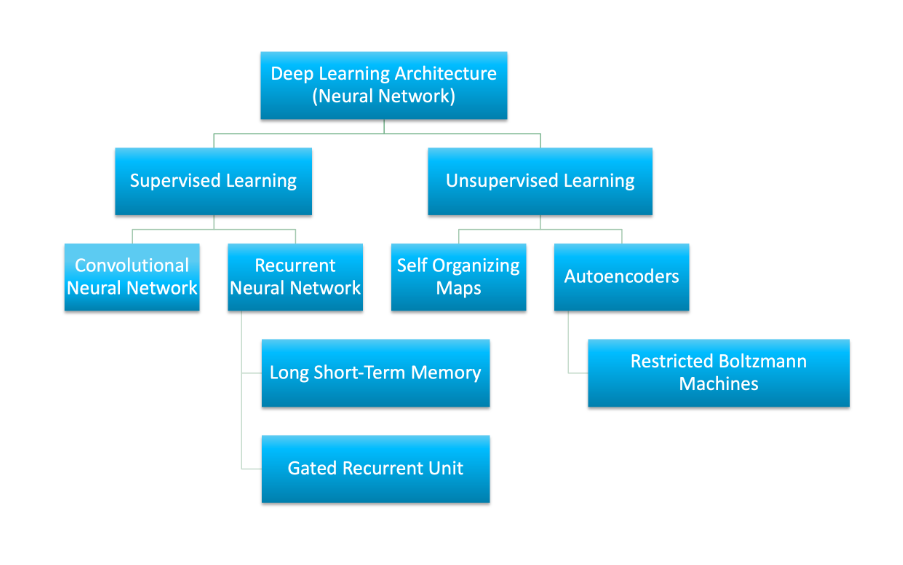
\includegraphics[width=1\textwidth]{DeepLearning_Arch.PNG}
    \caption{Deep learning architectures \cite{madhavan2017deep}}
\end{figure}
\begin{itemize}
    \item \textbf{Supervised deep learning: }
    Supervised learning refers to the problem space wherein the target to be predicted is clearly labeled within the data that is used for training.
    \begin{itemize}
        \item \textbf{Convolutional neural networks: } A CNN is a multilayer neural network used for image processing, inspired by the animal visual cortex. It was first created by Yann LeCun for recognizing handwritten characters. Early layers detect basic features, while subsequent layers combine these features to extract higher-level attributes of the input image. The LeNet CNN architecture performs feature extraction and classification through multiple layers, including convolutional and pooling layers, a fully connected multilayer perceptron, and an output layer. 
        \begin{figure}[H]
            \centering
            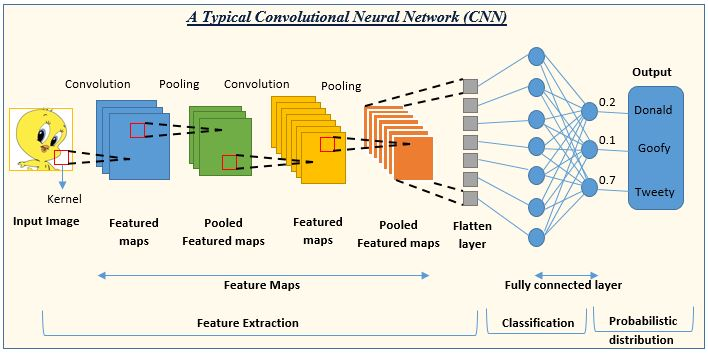
\includegraphics[width=0.8\linewidth]{tex/img/CNN.jpeg}
            \caption{Convolutional Neural Network \cite{Saily_Shah}}
            \label{fig:CNN}
        \end{figure}
        The network is trained through back-propagation. A Convolutional Neural Network (CNN) is a highly effective multilayer neural network that was inspired by the visual cortex of animals. It is primarily used for image processing applications. The first-ever CNN was created by Yann LeCun, which revolutionized the recognition of handwritten characters such as postal codes.
        
        With its deep network architecture, CNN can detect basic features, such as edges, through its initial layers and then combine these features to extract higher-level attributes of the input image.
        
        The LeNet CNN architecture, consisting of multiple layers that perform feature extraction and classification, is a prime example of CNN's effectiveness. It includes convolutional and pooling layers, a fully connected multilayer perceptron, and an output layer that identifies features of the image. The network is trained through back-propagation, making it an even more efficient tool. \cite{alzubaidi2021review} \cite{ansari2020building}
        
        \item  \textbf{The Gated Recurrent Unit (GRU) networks} In 2014, a simpler version of the LSTM network was introduced, known as the Gated Recurrent Unit (GRU). The GRU has two gates, an update gate and a reset gate, which replace the output gate present in the LSTM. The update gate determines how much of the previous cell contents should be kept, while the reset gate determines how to combine the new input with the previous cell contents. By setting the reset gate to 1 and the update gate to 0, a GRU can function as a standard RNN.\cite{madhavan2017deep}
        
        \begin{figure}[H]
            \centering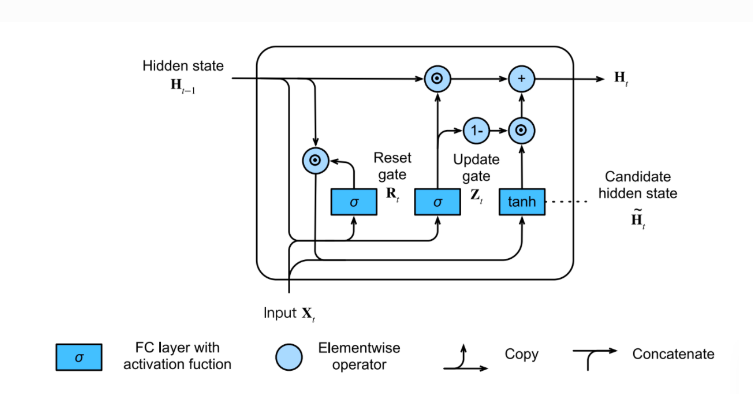
\includegraphics[width=1\textwidth]{GRU_layers.PNG}
            \caption{GRU networks \cite{bfortuner_mlglossary}}
        \end{figure}
        The LSTM is more expressive and can lead to better results with more data, while the GRU is simpler, can be trained more quickly, and can be more efficient in its execution.
    \end{itemize}

     \item \textbf{Recurrent Neural Network (RNN): } is a neural network that contains a hidden state which captures historical information up to the current timestep. The hidden state of the current state uses the same definition as the previous timestep, which makes the computation recurrent, hence its name.

    The RNN is a foundational network architecture from which other deep learning architectures are built. The primary difference between a typical multilayer network and an RNN is that an RNN may have connections that feed back into prior layers (or the same layer) instead of completely feed-forward connections. This feedback allows RNNs to retain memory of past inputs and model problems in time.
    
    RNNs include a rich set of architectures, and one popular topology is called Long Short-Term Memory (LSTM). The key differentiator is feedback within the network, which can appear from a hidden layer, the output layer, or some combination of both.
    
    RNNs can be unfolded over time and trained using standard backpropagation or a variant called backpropagation through time (BPTT).  \cite{sherstinsky2020fundamentals}\\
    \begin{figure}[H]
        \centering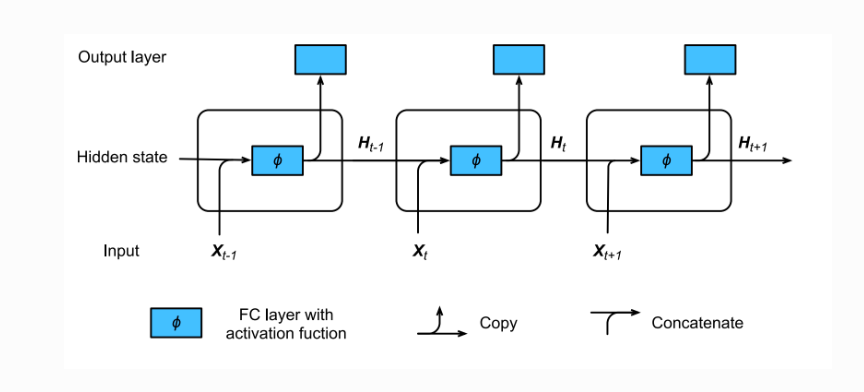
\includegraphics[width=0.8\textwidth]{RNN.PNG}
        \caption{Recurrent Neural Network \cite{bfortuner_mlglossary}}
    \end{figure}
    \item \textbf{Gated Recurrent Unit (GRU) Layer: } GRU supports: \\
    \textbf{hidden gate} the gating of hidden state, \\
    \textbf{Reset gate} controls how much of the previous hidden state we might still want to remember.\\
    \textbf{Update gate} controls how much of current hidden state is just a copy of the previous state
    The structure and math are as follow:
    \begin{figure}[H]
        \centering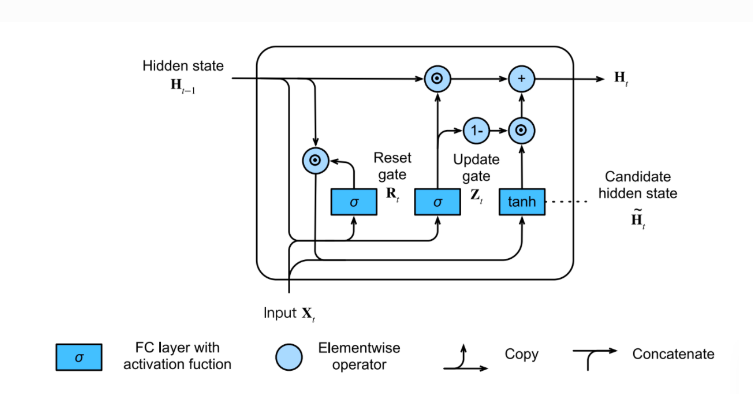
\includegraphics[width=0.8\textwidth]{GRU_layers.PNG}
        \caption{Gated Recurrent Unit \cite{bfortuner_mlglossary}}
    \end{figure}
    \item \textbf{Long short-term memory (LSTM): } Long Short-Term Memory (LSTM) is a type of recurrent neural network (RNN) architecture. It is specifically designed to address the vanishing gradient problem, which can occur in traditional RNNs. LSTMs are particularly useful for handling tasks that involve sequences of data, such as speech recognition, natural language processing, time series analysis, and more.

    The most remarkable feature of LSTMs is their ability to capture and remember long-term dependencies in sequential data while avoiding the vanishing gradient problem. This is a significant advantage over traditional RNNs, which can struggle with the training of long sequences. \cite{alzubaidi2021review} \cite{madhavan2017deep}
    
    Here are the main components and features of an LSTM:
    
    \textbf{Cell State (Ct):}
    
    The cell state in LSTM serves as a long-term memory. It remains unchanged throughout the chain of the LSTM network, with only some minor linear interactions. It works like a conveyor belt that runs through the entire sequence, and information can be added or removed from it as needed.\\
    
    \textbf{Hidden State (ht):}\\
    
    The hidden state in LSTM is essentially a short-term memory that plays a crucial role in capturing and retaining short-term dependencies in the sequence. It is determined by both the current input and the previous hidden state at each time step.\\
    \textbf{Input Gate: } 
    The input gate is responsible for determining the amount of newly received information that should be added to the cell state. It utilizes a sigmoid activation function to determine which values should be updated (values close to 1) and which values should be ignored (values close to 0).\\
    \textbf{Forget Gate: }
    The forget gate is responsible for determining which information from the cell state should be disregarded. It takes into account the previous hidden state and the current input to decide which parts of the cell state are no longer important. It utilizes a sigmoid activation function to produce output values ranging from 0 to 1.\\
    \textbf{Cell State Update: }
   Cell state update is determined by two gates - the input gate and the forget gate. These gates work together to decide what new information should be added to the cell state and what information should be removed from it. The input gate determines the new information to be stored, while the forget gate determines which information should be discarded.\\
    \textbf{Output Gate:}
    
    The output gate plays a crucial role in deciding the next hidden state. It utilizes two activation functions - sigmoid and tanh. Sigmoid determines which parts of the cell state should be outputted, while tanh generates a vector of new candidate values that are added to the hidden state.
    \href{https://ml-cheatsheet.readthedocs.io/en/latest/layers.html#lstm}{Layers}
    \begin{figure}[H]
        \centering
        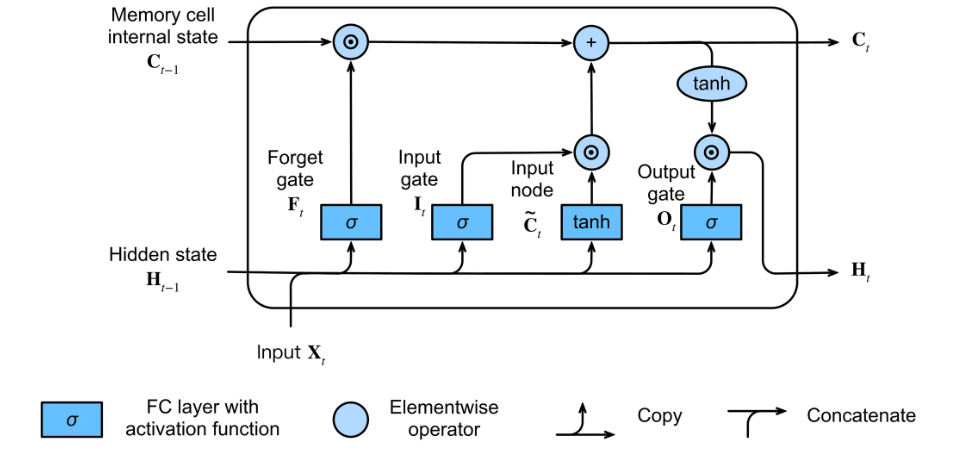
\includegraphics[width=0.8\linewidth]{tex/img/LSTM_layer.PNG}
        \caption{Long short-term memory \cite{yu2023popular}}
        \label{fig:LSTM_layer}
    \end{figure}
    \end{itemize}

\end{itemize}

\subsubsection{Section Unsupervised learning}

Unsupervised learning involves training models without target labels present within the data using unsupervised architectures.\cite{coates2011analysis}
\begin{itemize}
    \item \textbf{Self-organized maps: } Self-Organizing Maps (SOM) are a type of unsupervised neural network invented by Dr. Teuvo Kohonen in 1982, also known as Kohonen maps. Unlike traditional artificial neural networks, SOMs create clusters of input data by reducing input dimensionality. \cite{alzubaidi2021review}, \cite{madhavan2017deep}

    \begin{figure}[H]
        \centering
        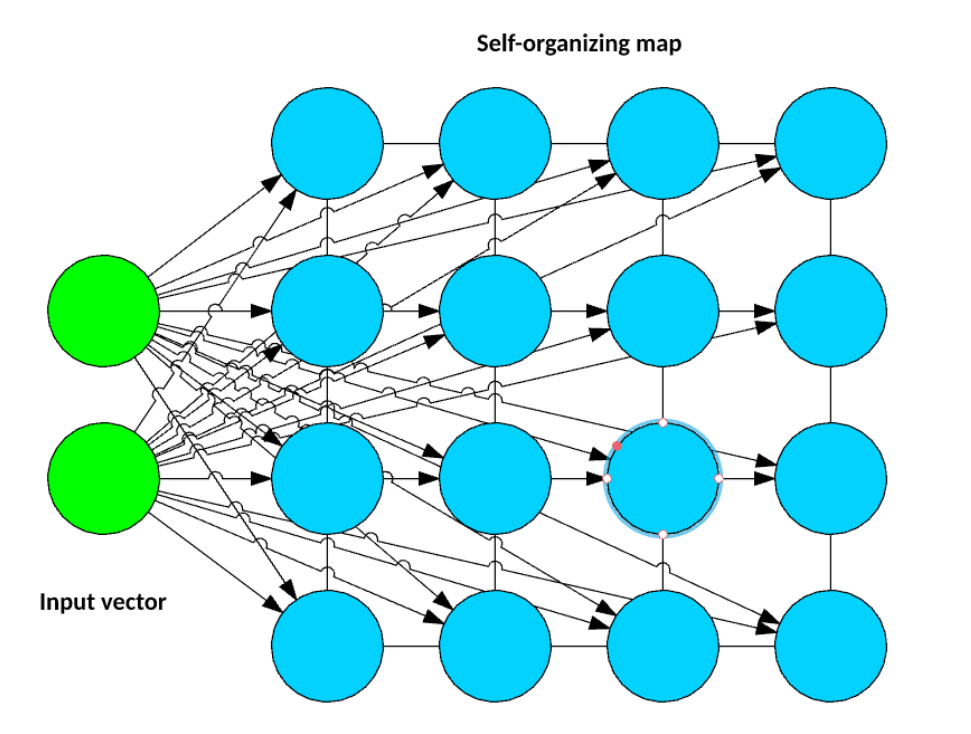
\includegraphics[width=0.5\textwidth]{Self_organizingMap.PNG}
        \caption{Self-organized map (SOM)}
        \label{fig:Self-organized map (SOM)}
    \end{figure}
    \textbf{Example applications:} Dimensionality reduction, clustering high-dimensional inputs to 2-dimensional output, radiant grade result, and cluster visualization
    \item \textbf{Autoencoders: } Autoencoders are a variant of artificial neural networks (ANNs) that consist of three layers: the input layer, the hidden layer, and the output layer. First, the input layer is encoded into the hidden layer using an appropriate encoding function. The number of nodes in the hidden layer is much less than the number of nodes in the input layer. This hidden layer contains a compressed representation of the original input. Finally, the output layer aims to reconstruct the input layer by using a decoder function.
    
    \begin{figure}[H]
        \centering
        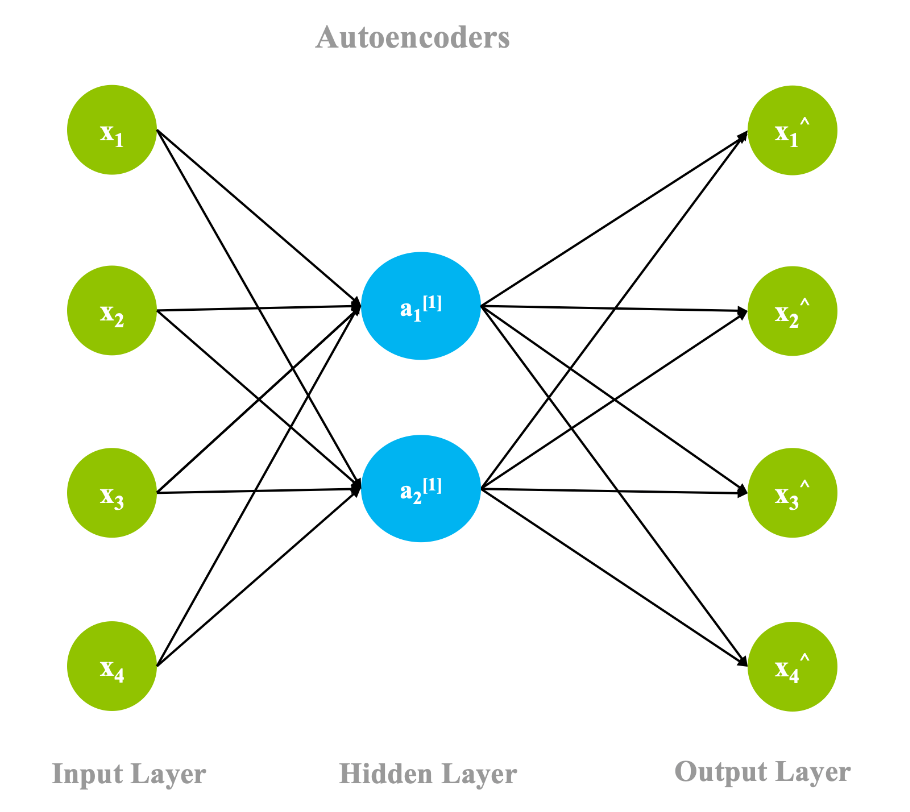
\includegraphics[width=0.7\linewidth]{tex/img/Autoencoders.PNG}
        \caption{Autoencoders \cite{madhavan2017deep}}
        \label{fig:Autoencoders}
    \end{figure}
   During the training phase, an error function is used to calculate the difference between the input and output layers, and the weights are adjusted accordingly to minimize the error. \\ 
    \textbf{Example applications:} Dimensionality reduction, data interpolation, and data compression/decompression.\\ 
    \item \textbf{Restricted Boltzmann Machines: } A Restricted Boltzmann Machine (RBM) is a type of neural network that consists of two layers: input and hidden layers. As depicted in figure \ref{fig:Restricted Boltzmann Machines}, every node in the hidden layer is connected to every node in the visible layer. Unlike traditional Boltzmann machines, where nodes in the input and hidden layers are interconnected, RBMs restrict the connections between nodes within a layer due to computational complexity.
    
    \begin{figure}[H]
        \centering
        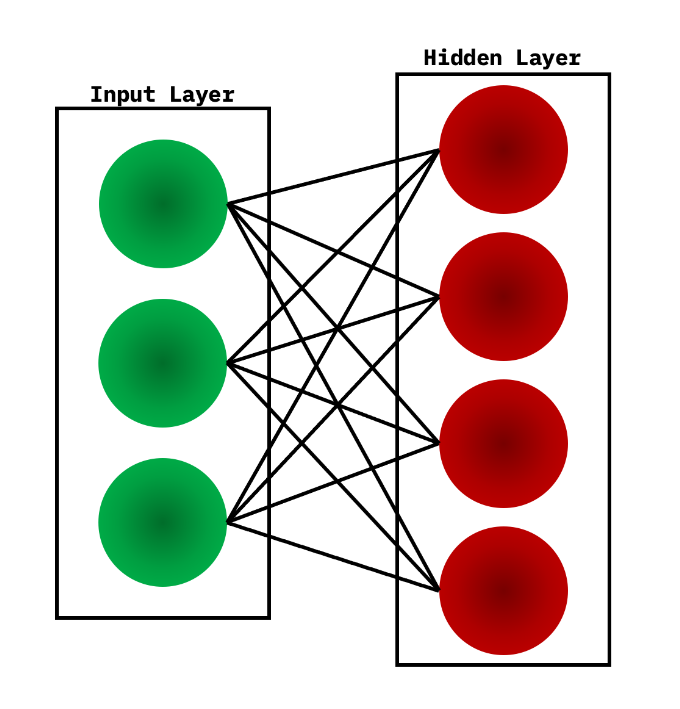
\includegraphics[width=0.6\textwidth]{RestrictedBoltzmannMachines.PNG}
        \caption{Restricted Boltzmann Machines \cite{madhavan2017deep}}
        \label{fig:Restricted Boltzmann Machines}
    \end{figure}
    During the training phase of RBMs, a stochastic approach is used to calculate the probability distribution of the training set. At the beginning of the training, each neuron is activated at random. The model also contains hidden and visible biases. The hidden bias is used in the forward pass to build the activation, while the visible bias helps in reconstructing the input. RBMs are also called generative models because the reconstructed input is always different from the original input. Additionally, due to the built-in randomness, the same predictions result in different outputs. RBMs is a deterministic model, and that makes it significantly different from Autoencoder. \cite{madhavan2017deep} \cite{alzubaidi2021review} \\
    \textbf{Example applications:} Dimensionality reduction and collaborative filtering.\\
    \item \textbf{Deep belief networks: } Deep belief networks (DBN) are multilayer networks that typically have several hidden layers, making them deep. Each pair of connected layers in a DBN is a Restricted Boltzmann Machine (RBM). The input layer of the DBN represents the raw sensory inputs, while each hidden layer learns abstract representations of this input. The output layer is treated differently and is responsible for network classification during training. The DBN is trained in two steps: unsupervised pretraining and supervised fine-tuning. \cite{sohn2021deep}, \cite{coates2011analysis}
    
    \begin{figure}[H]
        \centering
        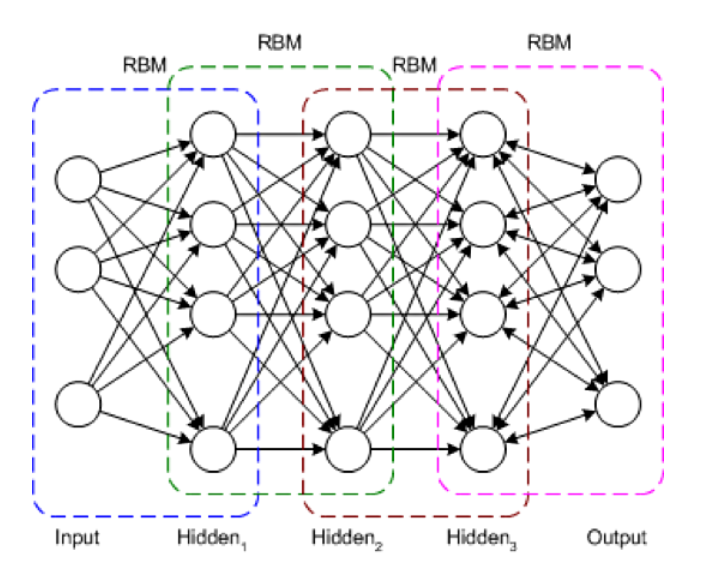
\includegraphics[width=0.7\textwidth]{DeepBelief_Networks.PNG}
        \caption{Deep belief networks architecture \cite{madhavan2017deep}}
        \label{fig:Deep belief networks}
    \end{figure}
    During unsupervised pretraining, each Restricted Boltzmann Machine (RBM) is trained to reconstruct its input. For instance, the first RBM reconstructs the input layer to the first hidden layer. Similarly, the next RBM is trained by using the outputs of the previous hidden layer as the inputs, and so on until each layer is pretrained. 

    After pretraining, fine-tuning commences, and the output nodes are assigned labels to give them meaning, i.e., to signify what they represent in the context of the network. The final step involves applying full network training using either gradient descent learning or back-propagation to complete the training process. \\
    \textbf{Applications: } object detection, information processing, natural language understanding processing, etc. \\
    \item \textbf{Deep stacking networks: } Deep stacking networks, also known as deep convex networks, are different from traditional deep learning frameworks. Although they consist of a deep network, they are actually a deep set of individual networks, each with its own hidden layers. 

    This architecture was developed to solve one of the main problems with deep learning: the complexity of training. Each layer in a deep learning architecture exponentially increases the complexity of training, but the DSN views training as a set of individual training problems, instead of a single problem.
    
    The DSN consists of a set of modules, each of which is a subnetwork in the overall hierarchy of the DSN. For example, in one instance of this architecture, three modules are created for the DSN. Each module consists of an input layer, a single hidden layer, and an output layer. Modules are stacked one on top of another, where the inputs of a module consist of the prior layer outputs and the original input vector. 
    
    This layering allows the overall network to learn more complex classifications than would be possible given a single module. \cite{deng2014tutorial}, \cite{madhavan2017deep}
    
    \begin{figure}[H]
        \centering
        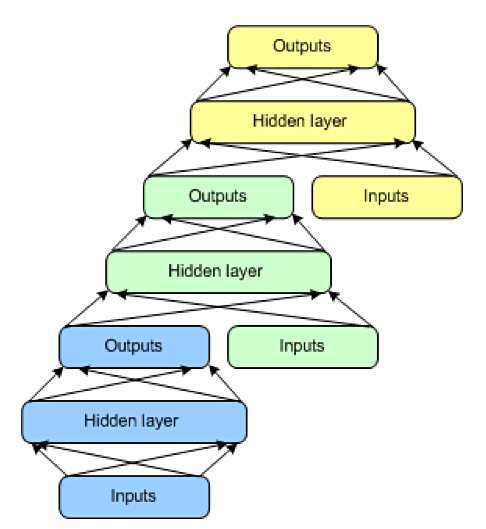
\includegraphics[width=0.5\textwidth]{DeepStackNetworks.PNG}
        \caption{Deep stacking networks architecture \cite{madhavan2017deep}}
        \label{fig:Deep stacking networks}
    \end{figure}
    \textbf{Example applications:} Information retrieval and continuous speech recognition
    

\end{itemize}
